% nie rusza�
\RequirePackage{ifpdf}
\newif\ifelektroniczna
\newif\ifjednostronna
\newif\ifprojektInzynierski

%%%%%%%%%%%%%%%%%%%%%%%%%%%%%%%%%%%%%%%%%%%%%%%%%%%%%%%%%%%%%%%%%%%%%%%%%%%%
% USTAWIENIA GLOBALNE I domy�lna �cie�ka do plik�w z obrazkami, kodowanie itp. 
% okre�lone s� w drugiej sekcji ustawie�

% czy projekt czy praca magisterska
\projektInzynierskitrue % projekt
%\projektInzynierskifalse % praca magisterska

% czy wersja elektroniczna (pdf z kolorowymi linkami) czy nie (np. do druku)
\elektronicznatrue
%\elektronicznafalse

% czy jednostronna (recenzent), czy dwustronna (do akt);
% UWAGA: to nie jest dyrektywa dla drukarki; nie zmienia sposobu wydruku, 
% tylko to, w jaki spos�b rozpoczynane s� rozdzia�y, ustawiane marginesy
% itp.

%\jednostronnafalse
\jednostronnatrue

%%%%%%%%%%%%%%%%%%%%%%%%%%%%%%%%%%%%%%%%%%%%%%%%%%%%%%%%%%%%%%%%%%%%%%%%%%%%


% nie rusza�
\ifjednostronna
    \def\strony{oneside,openany}
\else
    \def\strony{twoside,openright}
\fi

\ifpdf
    % uwaga, ustawiaj�c co� innego ni� 12 sprawd� uk�ad strony tytu�owej (marginesy)
    \documentclass[pdftex,12pt,a4paper,\strony,colorlinks,nocenter,noupper,crosshair]{thesis}
    \usepackage[pdftex]{graphicx}
    \pdfcompresslevel=1
\else    
    \documentclass[12pt,a4paper,\strony,nocenter,noupper,crosshair]{thesis}
    \usepackage{graphicx}
\fi

% nie rusza�
\usepackage{url}
\usepackage{stronatytulowa}

%%%%%%%%%%%%%%%%%%%%%%%%%%%%%%%%%%%%%%%%%%%%%%%%%%%%%%%%%%%%%%%%%%%%%%%%%%%%
% USTAWIENIA GLOBALNE - cz�� 2
%

% kodowanie dokumentu
%\usepackage[utf8]{inputenc}   % linuks/windows/mac; pozwala na �atwe mieszanie znak�w z r�nych j�zyk�w
\usepackage[cp1250]{inputenc} % windows

% dane 
\ifprojektInzynierski
    \def\rodzaj{Sprawozdanie z projektu z In�ynierii Programowania}
\else
    \def\rodzaj{Praca dyplomowa magisterska}
\fi
%\def\rodzaj{Praca przej�ciowa}

% stan na 2011-2012
\ifprojektInzynierski
    \def\wydzial{In�ynierii Biomedycznej}
\else
    \def\wydzial{In�ynierii Biomedycznej}
\fi

\def\tytul{Aplikacja webowa do komunikacji z lekarzem} % Prosz� u�y� i ma�ych, i du�ych liter!
\def\autor{Autorzy: 
D. Bara�ski, K. Bielecka, M. Cebrat, P. Wr�bel} %Jan Kowalski a NIE JAN KOWALSKI

% tytu� i autor dla pdfa - najcz�ciej jw, ale bez podzia�u na liniie i BEZ POLSKICH LITER
\def\tytulpdf{dawid_baranski_sprawozdanie}
\def\autorpdf{Dawid Baranski}

% promotor
\def\promotor{Prowadz�ca projekt: Dr in�. Joanna Czajkowska} % prof. nzw. dr hab. in�. dr n.med doc. Jan Kowalski

% z konsultantem/bez konsultanta
%\def\konsultant{Konsultant: Konsultant} prof. nzw. dr hab. in�. dr n.med doc. Jan Nowak
\def\konsultant{}

\def\data{Zabrze, maj, 2019} % uwaga na wielko�� liter: grudzie� 2012/czerwiec 2012/..

% do pdfa
\def\slowakluczowe{SLOWA,KLUCZOWE}

% �cie�ka do obrazk�w
\graphicspath{{./rysunki/}}

% ustawienia dla pdfa
\ifpdf
\ifelektroniczna
     \usepackage[pdfusetitle=true,
	  pdfsubject={\tytulpdf},
	        pdfkeywords={\slowakluczowe}, 
		pdfcreator={\autorpdf},
		pdfstartview=FitV,
		linkcolor=blue,
		citecolor=red,
		]{hyperref}
\fi                 
\fi


\usepackage{layout}% poka� marginesy

% Nazwa za��cznik�w 
\def\appendixname{Za��cznik}
%%%%%%%%%%%%%%%%%%%%%%%%%%%%%%%%%%%%%%%%%%%%%%%%%%%%%%%%%%%%%%%%%%%%%%%%%%%%

% nie rusza� (cho� chwilowo niepotrzebne)
%	\author{\autor}
%	\title{\tytul}
%	\date{\data}
%

% === PAKIETY ===
\usepackage{url}

% �adne czcionki dla PDF + ustawienia spolszczaj�ce
\usepackage{t1enc,amsmath}
\usepackage[OT4,plmath]{polski}

% potrzebne dla strony tytu�owej:
\usepackage{helvet} 

% pierwszy paragraf w rozdziale/sekcji powinien by� wci�ty
\usepackage{indentfirst}

% marginesy
%\usepackage{anysize}
%\marginsize{3cm}{2.5cm}{2.5cm}{2.5cm}%LPGD
%\setlength{\textheight}{24cm}
% za spraw� thesis
%\textwidth 150mm
%\textheight 225mm

% czcionki matematyczne
\usepackage{amsfonts}

% rysunki z�o�one z wielu [pod]rysunk�w
\usepackage{subfig}
\captionsetup[subfigure]{justification=centerfirst}

% mo�liwo�� sklejania wierszy tabeli
\usepackage{multirow}

% mo�liwo�� wklejania adres�w - jest ju� w��czony wy�ej
%\usepackage{url}

% ulepszona obs�uga cytowa�
\usepackage{cite}

% listingi
\usepackage{listings}
% domy�lne ustawienia (niestety utf8 nie jest akceptowany)
%\lstset{language={Matlab},inputencoding=cp1250}}
%\lstset{language={Matlab},inputencoding=latin2}}
\lstset{language={Java},inputencoding=latin2} % powinno pasowa� te� do C#

% \addcontentsline nie dzia�a za dobrze w po��czeniu z hyperref, ale to nie dzia�a z klas� thesis
%\usepackage[nottoc]{tocbibind}

% strona po cleardoublepage powinna by� pusta, nie z nag��wkami
\usepackage{cleardpempty}

% == opcjonalne

% wymu� po�o�enie grafiki (itp.) przez [H]
\usepackage{float} 

% znak promila i inne znaki specjalne
%\usepackage{textcomp}

% je�li trzeba obr�ci� stron� (wstawi� co� w orientacji poziomej), u�yj tych pakiet�w
%\ifpdf\usepackage{pdflscape}\else\usepackage{lscape}\fi

% je�li potrzebujesz d�ugich tabeli (wiele stron)
%\usepackage{longtable}

% === POLECENIA DODATKOWE ===

% wektor w tek�cie
\def\vec#1{\ensuremath{\mathbf{#1}}}

% anglicyzmy i �acinizmy
\def\ang#1{ang.~\emph{#1}}
\def\lat#1{�ac.~\emph{#1}}

% proste e (jako podstawa logarytmu naturalnego) we wzorach i w tek�cie:
\def\e{\ensuremath{\textrm{\normalfont{}e}}}

% znak stopnia [jak w "5 stopni"]
\def\stopien{\ensuremath{^{\circ}}\protect\space}

% notatki na marginesie
\def\fixme#1{\marginpar{\tiny{}#1}}
%\def\fixme#1{} % gdy nie chcemy ich drukowa�, wystarczy zast�pi� powy�sze tym

%ODNOSNIKI 
% �eby wykorzysta� przypis dwukrotnie; druga wersja gorzej dzia�a�a w po��czeniu 
% z hyperref; czyli \footnote{blablabla \label{przypisX}} + \footnotereuse{przypisX}
%\newcommand{\footnreuse}[1]{\raisebox{1ex}{\scriptsize{}\protect\ref{#1}}}

% == �RODOWISKA DLA TWIERDZE�, LEMAT�W itp. ===
\newtheorem{twierdzenie}{Twierdzenie}[chapter]
\newtheorem{wlasnosc}{W�asno��}[chapter]
\newtheorem{lemat}{Lemat}[chapter]
\newenvironment{dowod}{\parindent=0pt{\bf Dow�d. }}{\begin{flushright}$\square$\end{flushright}}

% === RACZEJ NIE RUSZA� ===

%\usepackage{makeidx}
%\makeindex
%\usepackage{threeparttable}
%\usepackage[small,center]{caption2}

\def\captionlabeldelim{.}

%\usepackage{geometry}
%GATHER{thesis.bib}
%\usepackage[twoside]{geometry}
%\geometry{ lmargin=3.5cm, rmargin=2.5cm, tmargin=3cm, bmargin=3cm,
%headheight=1cm, headsep=0.5cm, footskip=0pt }

\linespread{1}
\chapterfont{\Huge\bfseries}
\sectionfont{\bfseries\Large}
\subsectionfont{\bfseries\large}
\institutionfont{\bfseries}%\mdseries}
\def\captionlabelfont{\bfseries}

\renewcommand{\figureshortname}{Rys.}
\renewcommand{\tableshortname}{Tab.}

\renewcommand\floatpagefraction{.9}
\renewcommand\topfraction{.9}
\renewcommand\bottomfraction{.9}
\renewcommand\textfraction{.1}
\setcounter{totalnumber}{50}
\setcounter{topnumber}{50}
\setcounter{bottomnumber}{50}

\newcommand{\topcaption}{%                  % robi podpis nad tabelk� z odst�pem po podpisie
   \setlength{\abovecaptionskip}{0pt}%
   \setlength{\belowcaptionskip}{10pt}%
   \caption}



% marginesy
\usepackage{anysize}
\marginsize{3cm}{2.5cm}{2.5cm}{2.5cm}%LPGD
%\setlength{\textheight}{24cm}
% za spraw� thesis
%\textwidth 150mm
%\textheight 225mm

\begin{document}
%
\bibliographystyle{acm}
%

%
\stronatytulowa
\titlepage
%-\cleardoublepage % je�li dwustronnie, to druga strona powinna by� pusta
\frontmatter 
%\maketitle

%\tocbibname

\tableofcontents \listoffigures \listoftables
%\listofacros
%\input{abbrev_body}
%\newpage
%\input{spis_oznaczen}

\mainmatter % <--- to + frontmatter powy�ej odpowiada za fakt, �e numerowanie jest od 1!
\renewcommand{\arraystretch}{1.2}

\chapter{Wst�p}
\section{Cel projektu}
Celem niniejszej pracy by�o utworzenie aplikacji webowej, wspomagaj�cej kontakt pomi�dzy lekarzem, a pacjentem. Docelowo, aplikacja powinna umo�liwia� wymian� danych na bie��co. Pacjent powinien mie� mo�liwo�� rozpocz�cia rozmowy z wszystkimi lekarzami dost�pnymi on--line. Za�o�ono, i� aplikacja stanowi narz�dzie, wspomagaj�ce prac� istniej�cej ju� przychodni lekarskiej.

Osi�gni�cie celu wymaga�o realizacji nast�puj�cych etap�w:
\begin{itemize}
\item przydzia�u zada� poszczeg�lnym osobom w grupie,
\item wyboru narz�dzi,
\item opracowania architektury bazy danych,
\item stworzenia interfejsu u�ytkownika,
\item implementacji poszczeg�lnych funkcjonalno�ci.
\end{itemize}
\section{Platforma projektowa}
\subsection{Angular}
Otwarty framework i platforma do tworzenia SPA, napisany w j�zyku TypeScript i wspierany oraz rozwijany przez Google.

Elementy Angular:
\begin{itemize}
\item architektura MVW - aplikacje mog� by� oparte o r�ne wzorce architektoniczne, z kt�rymi Angular sobie poradzi;
\item wstrzykiwanie zale�no�ci - wprowadzone przez nas funkcjonalno�ci w kodzie staj� si� bardziej zautomatyzowane;
\item modu�y - modu� jest podstawowym no�nikiem danych tak jak klasa, jednak nie mo�emy tworzy� instacji modu�u, opiera si� on na nieco innej funkcjonalno�ci;
\item dwukierunkowe wi�zanie danych - mechanizm dwukierunkowego wi�zania danych zapewnia dynamiczn� synchronizacj� danych mi�dzy warstw� widoku, a warstw� modelu danych;
\item nawigacja - mo�liwo�� przekierowywania, ingerowania w wy�wietlanie widoku strony dla odpowiedniego adresu;
\item filtrowanie danych - Angular oferuje wbudowane mechanizmy filtrowania, kt�re poniek�d wyr�czaj� deweloper�w od pisania w�asnych funkcji filtruj�cych dane.

\end{itemize}
\subsection{Firebase}
Jest to BaaS odpowiedzialny za nasz� architektur� backendow�, za marketing, monitoring wydajno�ci, zarz�dzanie uploadowanymi plikami, testowanie, modyfikowanie aplikacji i przechowywanie w bezpieczny spos�b.
\subsection{JSON}
Jest prostym formatem wymiany danych. Jego definicja opiera si� o podzbi�r j�zyka programowania JavaScript, Standard ECMA-262 3rd Edition - December 1999. JSON jest formatem tekstowym, ca�kowicie niezale�nym od j�zyk�w programowania, ale u�ywa konwencji, kt�re s� znane programistom korzystaj�cym z j�zyk�w z rodziny C.


JSON powsta� w oparciu o dwie struktury:
\begin{itemize}
\item Zbi�r par nazwa/warto��. W r�nych j�zykach jast to implementowane jako obiekt, rekord, struktura, s�ownik, tabela hash, lista z kluczem, albo tabela asocjacyjna.
\item Uporz�dkowana lista warto�ci. W wi�kszo�ci j�zyk�w implementuje si� to za pomoc� tabeli, wektora, listy, lub sekwencji.

\end{itemize}

Wspomniane struktury danych s� uniwersalne. Prawie wszystkie nowoczesne j�zyki programowania pos�uguj� si� nim w tej lub innej formie. Ma to sens, by format danych, kt�ry jest przeno�ny pomi�dzy r�nymi j�zykami programowania opiera� swoj� budow� na wspomnianych strukturach.

\section{Harmonogram prac}
\begin{table}[]
\centering
\caption{Harmonogram prac.}
\label{harmonogram}
\begin{tabular}{|l|l|}
\hline
\textbf{Termin} & \textbf{Wykonane prace}                                                                                                                                                      \\ \hline
26.02.2019       & Ustalenie tematu projektowego                                                                                                                                                \\ \hline
12.03.2019      & \begin{tabular}[c]{@{}l@{}}Zdefiniowanie problemu\\   Wyb�r kierownika projektu \\   Wyb�r platformy projektowej\end{tabular}                                                \\ \hline
26.03.2019      & \begin{tabular}[c]{@{}l@{}}analiza rynku\\   opracowanie architektury\\   systemu\\   zdefiniowanie\\   funkcjonalno�ci\\   schematy u�ycia\\   projekt GUI\end{tabular}     \\ \hline
09.04.2019      & \begin{tabular}[c]{@{}l@{}}zamockowanie bazy danych\\   Utworzenie ekranu logowania\\   i logiki\\   Utworzenie bazy danych\\   lek�w\\   wczytanie listy lek�w\end{tabular} \\ \hline
07.05.2019      & \begin{tabular}[c]{@{}l@{}}implementacja czatu\\   wczytanie listy lekarzy/pacjent�w\end{tabular}                                                                            \\ \hline
21.05.2019      & \begin{tabular}[c]{@{}l@{}}Implementacja dodawania lek�w\\   Walidacja logowania\end{tabular}                                                                                \\ \hline
04.06.2019      & \begin{tabular}[c]{@{}l@{}}Dokumentacja\\   Testowanie\\   Dodanie historii chor�b\end{tabular}                                                                              \\ \hline
\end{tabular}
\end{table}

Harmonogram prac zosta� przedstawiony w tabeli (Tab.~\ref{harmonogram}).

\section{Przegl�d rynku}
\subsection{Doktormed}
\begin{figure}[!htb]
	\centering
	
\includegraphics[width=.8\textwidth]{rynek1}
	\caption{Doktormed.}\label{l:rynek1}
\end{figure}

Jest to platforma umo�liwiaj�ca zadawanie pyta� do grona lekarzy w spos�b anonimowy, koszt porady to 50 z�otych i otrzymujemy odpowiedz od specjalisty z dziedziny zadanego przez nas pytania (Rys.~\ref{l:rynek1}). 

\subsection{Edoktor24}
\begin{figure}[!htb]
	\centering
	
\includegraphics[width=.8\textwidth]{rynek2}
	\caption{Edoktor24.}\label{l:rynek2}
\end{figure}

Jest to platforma umo�liwiaj�ca zadnie pyta� przez wybranie specjalisty zadanie pytania do kt�rego jest mo�liwe do��czenie wynik�w bada� a nast�pnie po wniesieniu op�aty otrzymujemy odpowiedz w ci�gu 24 godzin.  Mo�liwe s� tak�e konsultacje telefoniczne lub wideo konsultacje z wybranym specjalist� (Rys.~\ref{l:rynek2}).

\subsection{Grupa Luxmed}
\begin{figure}[!htb]
	\centering
	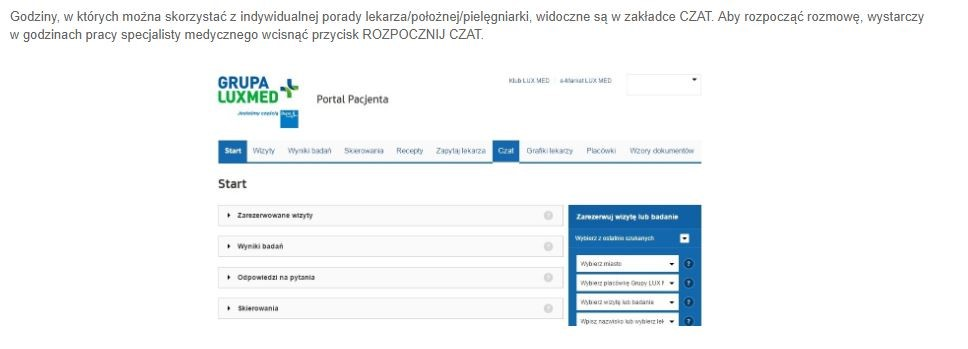
\includegraphics[width=.8\textwidth]{rynek3}
	\caption{Grupa Luxmed.}\label{l:rynek3}
\end{figure}

Jest to platforma umo�liwiaj�ca czat z piel�gniarkami lub lekarzami wybranych specjalizacji w wyznaczonym czasie kiedy s� dost�pni (Rys.~\ref{l:rynek3}).

\subsection{Kardiologonline}
\begin{figure}[!htb]
	\centering
	
\includegraphics[width=.8\textwidth]{rynek4}
	\caption{Kardiologonline.}\label{l:rynek4}
\end{figure}

Jest to platforma umo�liwiaj�ca um�wienie si� na konsultacje z wybranym specjalist� kt�re odb�d� si� za pomoc� menad�era lub facebooka (Rys.~\ref{l:rynek4}).

\subsection{Medicover}

\begin{figure}[!htb]
	\centering
	
\includegraphics[width=.8\textwidth]{rynek5}
	\caption{Medicover.}\label{l:rynek5}
\end{figure}

Jest to czat dost�pny za pomoc� przegl�darki internetowej w kt�rym pacjent mo�e otrzyma� odpowiedz na proste zadane pytanie do lekarza (Rys.~\ref{l:rynek5}).

\chapter{System}
\section{Architektura systemu}
\begin{figure}[!htb]
	\centering
	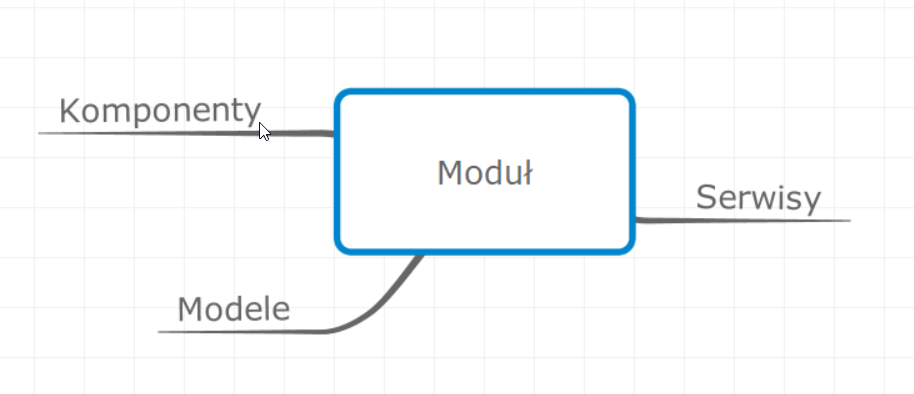
\includegraphics[width=.8\textwidth]{system-modul}
	\caption{Podzia� modu�u w Angular.}\label{l:system-modul}
\end{figure}

Framework Angular pomaga utrzyma� architektur� zgodn� z praktykami dobrego programowania. Aplikacja dzieli si� na modu�y, co jest odzwierciedleniem wzorca MVC (Rys.~\ref{l:system-modul}).

\begin{figure}[!htb]
	\centering
	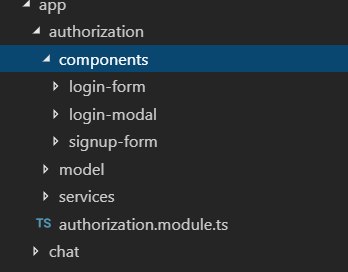
\includegraphics[width=.5\textwidth]{system-vsc}
	\caption{Podzia� modu�u w Angular.}\label{l:system-vsc}
\end{figure}

Przyk�adowa implementacja modu�u autoryzacji zosta�a przedstawiona na rysunku (Rys.~\ref{l:system-vsc}).

\begin{figure}[!htb]
	\centering
	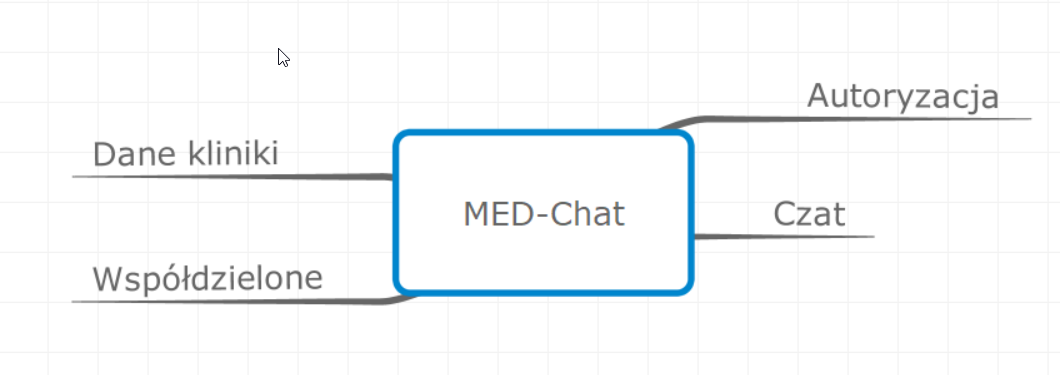
\includegraphics[width=.8\textwidth]{system}
	\caption{Architektura systemu.}\label{l:system}
\end{figure}

Aplikacja zosta�a podzielona na 4 g��wne modu�y, wed�ug funkcjonalno�ci. Jest to g��wna architektura systemu (Rys.~\ref{l:system}). 

\begin{figure}[!htb]
	\centering
	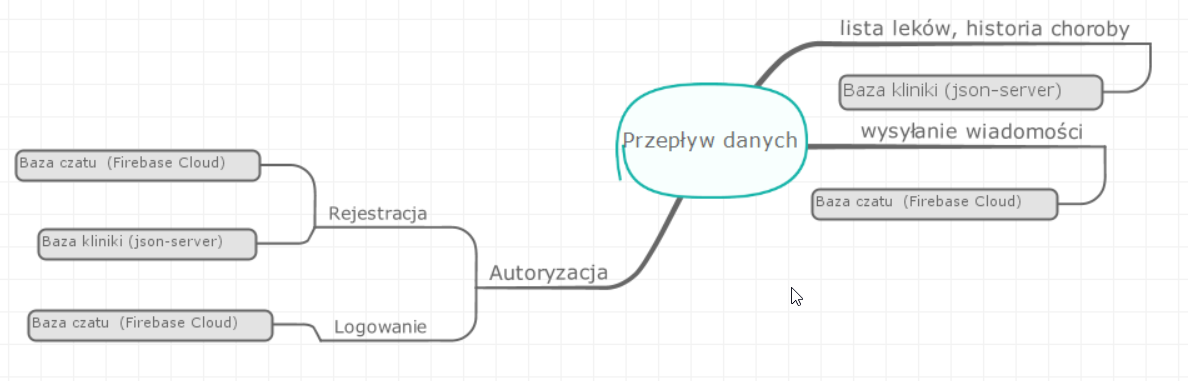
\includegraphics[width=1.1\textwidth]{system-przeplyw}
	\caption{Podzia� modu�u w Angular.}\label{l:system-przeplyw}
\end{figure}

Aplikacja pobiera dane z bazy danych kliniki. S� to informacje o danych osobowych u�ytkownika, historia stosowanych lek�w oraz przebytych chor�b. Baza ta zosta�a napisana w formacie json i jest kompilowana za po�rednictwem biblioteki \textit{json-server}, kt�ra jest na licencji \textit{Open-source}. Mo�na j� znale�� w serwisie \textit{Github} pod adresem https://github.com/typicode/json-server. Api do bazy danych zosta�o opublikowane za pomoc� \textit{Microsoft Azure}. 

Do logowania oraz obs�ugi czatu u�yto bazy danych \textit{Firebase Cloud}. Dzi�ki niej mo�liwe jest pisanie i odbieranie wiadomo�ci w czasie rzeczywistym.  

Dok�adny przep�yw danych w aplikacji zosta� przedstawiony na rysunku (Rys.~\ref{l:system-przeplyw}).

\section{Funkcje wewn�trzne}
Zachowanie i podzia� na funkcje wewn�trzne aplikacji, najlepiej opisuje podzia� na komponenty wewn�trz modu��w. W tej sekcji zosta�y opisane obowi�zki poszczeg�lnych komponent�w.

\begin{figure}[!htb]
	\centering
	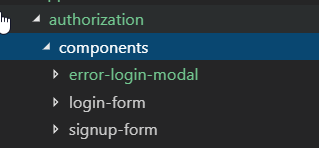
\includegraphics[width=.8\textwidth]{funkcje-auth}
	\caption{Komponenty modu�u autoryzacji.}\label{l:funkcje-auth}
\end{figure}
\subsection{Komponenty modu�u autoryzacji}


Modu� autoryzacji zawiera 4 komponenty (Rys.~\ref{l:funkcje-auth}):
\begin{itemize}
\item \textit{error-login-modal} - wy�wietlanie b��du podczas pr�by logowania z b��dnym loginem lub has�em,
\item \textit{login-form} - formularz logowania,
\item \textit{signup-form} - formularz rejestracji,
\end{itemize}


\begin{figure}[!htb]
	\centering
	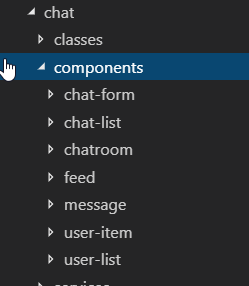
\includegraphics[width=.4\textwidth]{funkcje-chat}
	\caption{Komponenty modu�u czatu.}\label{l:funkcje-chat}
\end{figure}



\subsection{Komponenty modu�u czatu}

Modu� czatu zawiera 6 komponent�w (Rys.~\ref{l:funkcje-chat}):
\begin{itemize}
\item \textit{chatroom} - g��wne okienko czatu, zawieraj�ce wszystkie pozosta�e komponenty czatu;
\item \textit{chat-form} - formularz nowej wiadomo�ci,
\item \textit{feed} - wy�wietlenie wiadomo�ci czatu,
\item \textit{message} - wy�wietlenie pojedynczej wiadomo�ci,
\item \textit{user-list} - wy�wietlenie listy u�ytkownik�w,
\item \textit{user-item} - wy�wietlenie pojedynczego u�ytkownika.
\end{itemize}

\section{Przypadki testowe}

Przetestowano aplikacj� przez opisywanie zachowania programu w formie historyjek u�ytkownika (ang. user stories).  Zachowanie programu opisane jest w schemacie \textit{Given, When, Then}. Skutkuje to otrzymaniem jednoznacznie sprawdzalnych przypadk�w testowych.
Wykonane testy akceptacyjne z�o�one s� z trzech sekcji.
\begin{itemize}
\item \textit{Given} jest r�wnoznaczna z warunkami pocz�tkowymi,
\item \textit{When} jest to akcja do wykonania,
\item \textit{Then} prezentuje oczekiwany rezultat.
\end{itemize}



%Testowanie dotyczy funkcjonalno�ci zwi�zanej z obszarem �wicze�.
\subsubsection{Test 1}

\textbf{Given:} widok logowania. Wprowadzenie loginu i b��dnego has�a,


\textbf{when:} u�ytkownik naciska przycisk ,,Zaloguj",


\textbf{then:} powinien wy�wietli� si� komunikat ,,B��d logowania".

\subsubsection{Test 2}

\textbf{Given:} widok logowania. Wprowadzenie poprawnego loginu i has�a,


\textbf{when:} u�ytkownik naciska przycisk ,,Zaloguj",


\textbf{then:} powinien wy�wietli� si� g��wny widok czatu.



\subsubsection{Test 3}

\textbf{Given:} widok czatu. Wprowadzenie tre�ci wiadomo�ci,

\textbf{when:} u�ytkownik naciska przycisk ,,Wy�lij",

\textbf{then:} wiadomo�� powinna wy�wietli� si� w polu konwersacji.

\subsubsection{Test 4}

\textbf{Given:} obszar listy u�ytkownik�w,

\textbf{when:} u�ytkownik naciska element listy,

\textbf{then:} element powinien zosta� pod�wietlony na niebiesko.

\subsubsection{Test 5}

\textbf{Given:} obszar listy u�ytkownik�w,

\textbf{when:} u�ytkownik naciska element listy, zawieraj�cego imi� i nazwisko,

\textbf{then:} w nag��wku konwersacji powinno wy�wietli� si� imi� i nazwisko wybranej z listy osoby.

\subsubsection{Test 6}

\textbf{Given:} obszar listy lek�w,

\textbf{when:} u�ytkownik naciska element listy,

\textbf{then:} powinien zosta� wy�wietlony komunikat ze szczeg�owymi informacjami.

\subsubsection{Test 7}

\textbf{Given:} komunikat ze komunikat ze szczeg�owymi informacjami o leku,

\textbf{when:} u�ytkownik naciska przycisk ,,OK",

\textbf{then:} komunikat przestaje by� widoczny.

\subsubsection{Test 8}

\textbf{Given:} obszar historii chor�b,

\textbf{when:} u�ytkownik naciska element listy,

\textbf{then:} element powinien zosta� powi�kszony o dodatkowe informacje.


\chapter{Wnioski}
Cel pracy zosta� osi�gni�ty, gdy� utworzono aplikacj�, umo�liwiaj�c� bezpo�redni kontakt pomi�dzy pacjentem a lekarzem, bez konieczno�ci wcze�niejszego planowania wizyty. Dzi�ki wykorzystaniu najnowszych technologii, utworzono us�ug� �wiadczenia opieki zdrowotnej na odleg�o��. 
Do najwa�niejszych zalet powsta�ej aplikacji zalicza si�:
\begin{itemize}
\item zmniejszenie koszt�w opieki medycznej,
\item dost�p do lekarzy bez d�ugiego czasu oczekiwania na wizyt�,
\item kontakt z personelem medycznym w czasie urlopu,
\item szybkie konsultacje lekarskie -- mo�liwo�� poruszenia pilnych temat�w, wymagaj�cych weryfikacji osoby do�wiadczonej,
\item mo�liwo�� podgl�du przepisanych lek�w,
\item zredukowana liczba koniecznych dojazd�w do plac�wki,
\item szybki i �atwy dost�p do historii chor�b zar�wno ze strony lekarza, jak i od strony u�ytkownika.
\end{itemize}

W przysz�o�ci, aplikacja mo�e zosta� rozbudowana o kolejne modu�y, zwi�kszaj�ce funkcjonalno��. Mo�na stworzy� przydzia� danego lekarza do specjalizacji, mo�liwo�� wysy�ania za��cznik�w lub przeprowadzania rozm�w wideo.
%\begin{figure}[!htb]
%	\centering
%	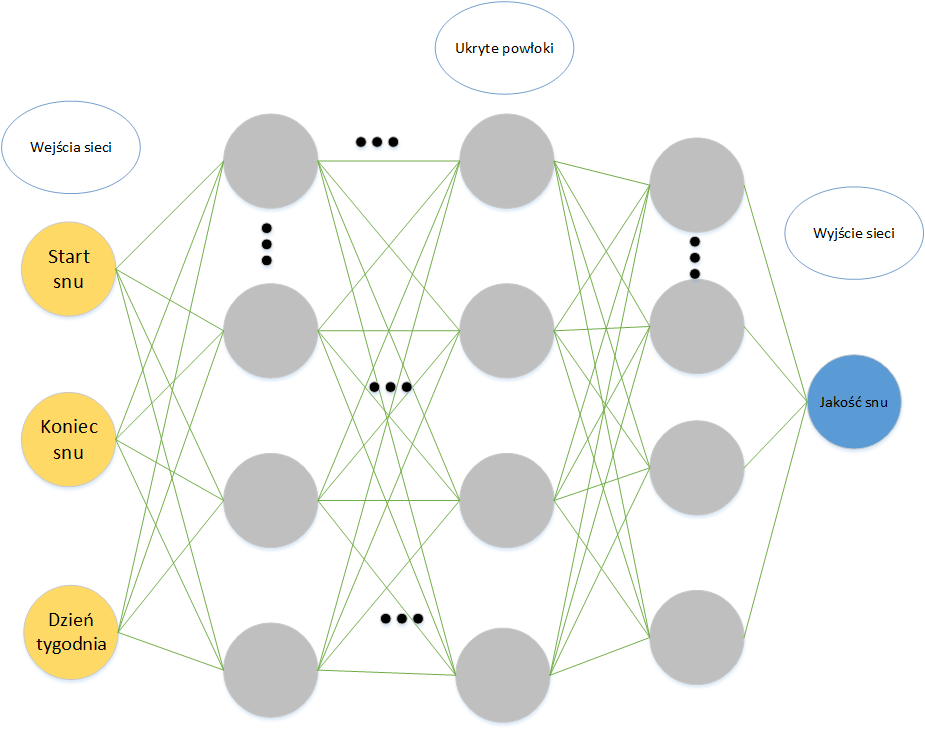
\includegraphics[width=1\textwidth]{lstm_schema}
%	\caption{Zaprojektowana sie� neuronowa.}\label{lstm-schema}
%\end{figure}

\begin{thebibliography}{999}


\end{thebibliography}




%\appendix  % <--- zaczynaj� si� dodatki; jak nazywa si� rozdzia� -> szuka� appendixname powy�ej

\clearpage 
%\addcontentsline{toc}{chapter}{\bibname}
%\bibliography{Praca}
%\nocite{deepl}
%\nocite{perceptron}
%\nocite{nardeas}
%\nocite{youtube}

\end{document}
